\hypersetup{pageanchor=false}
\begin{titlepage}
  \newgeometry{margin = 0in}
  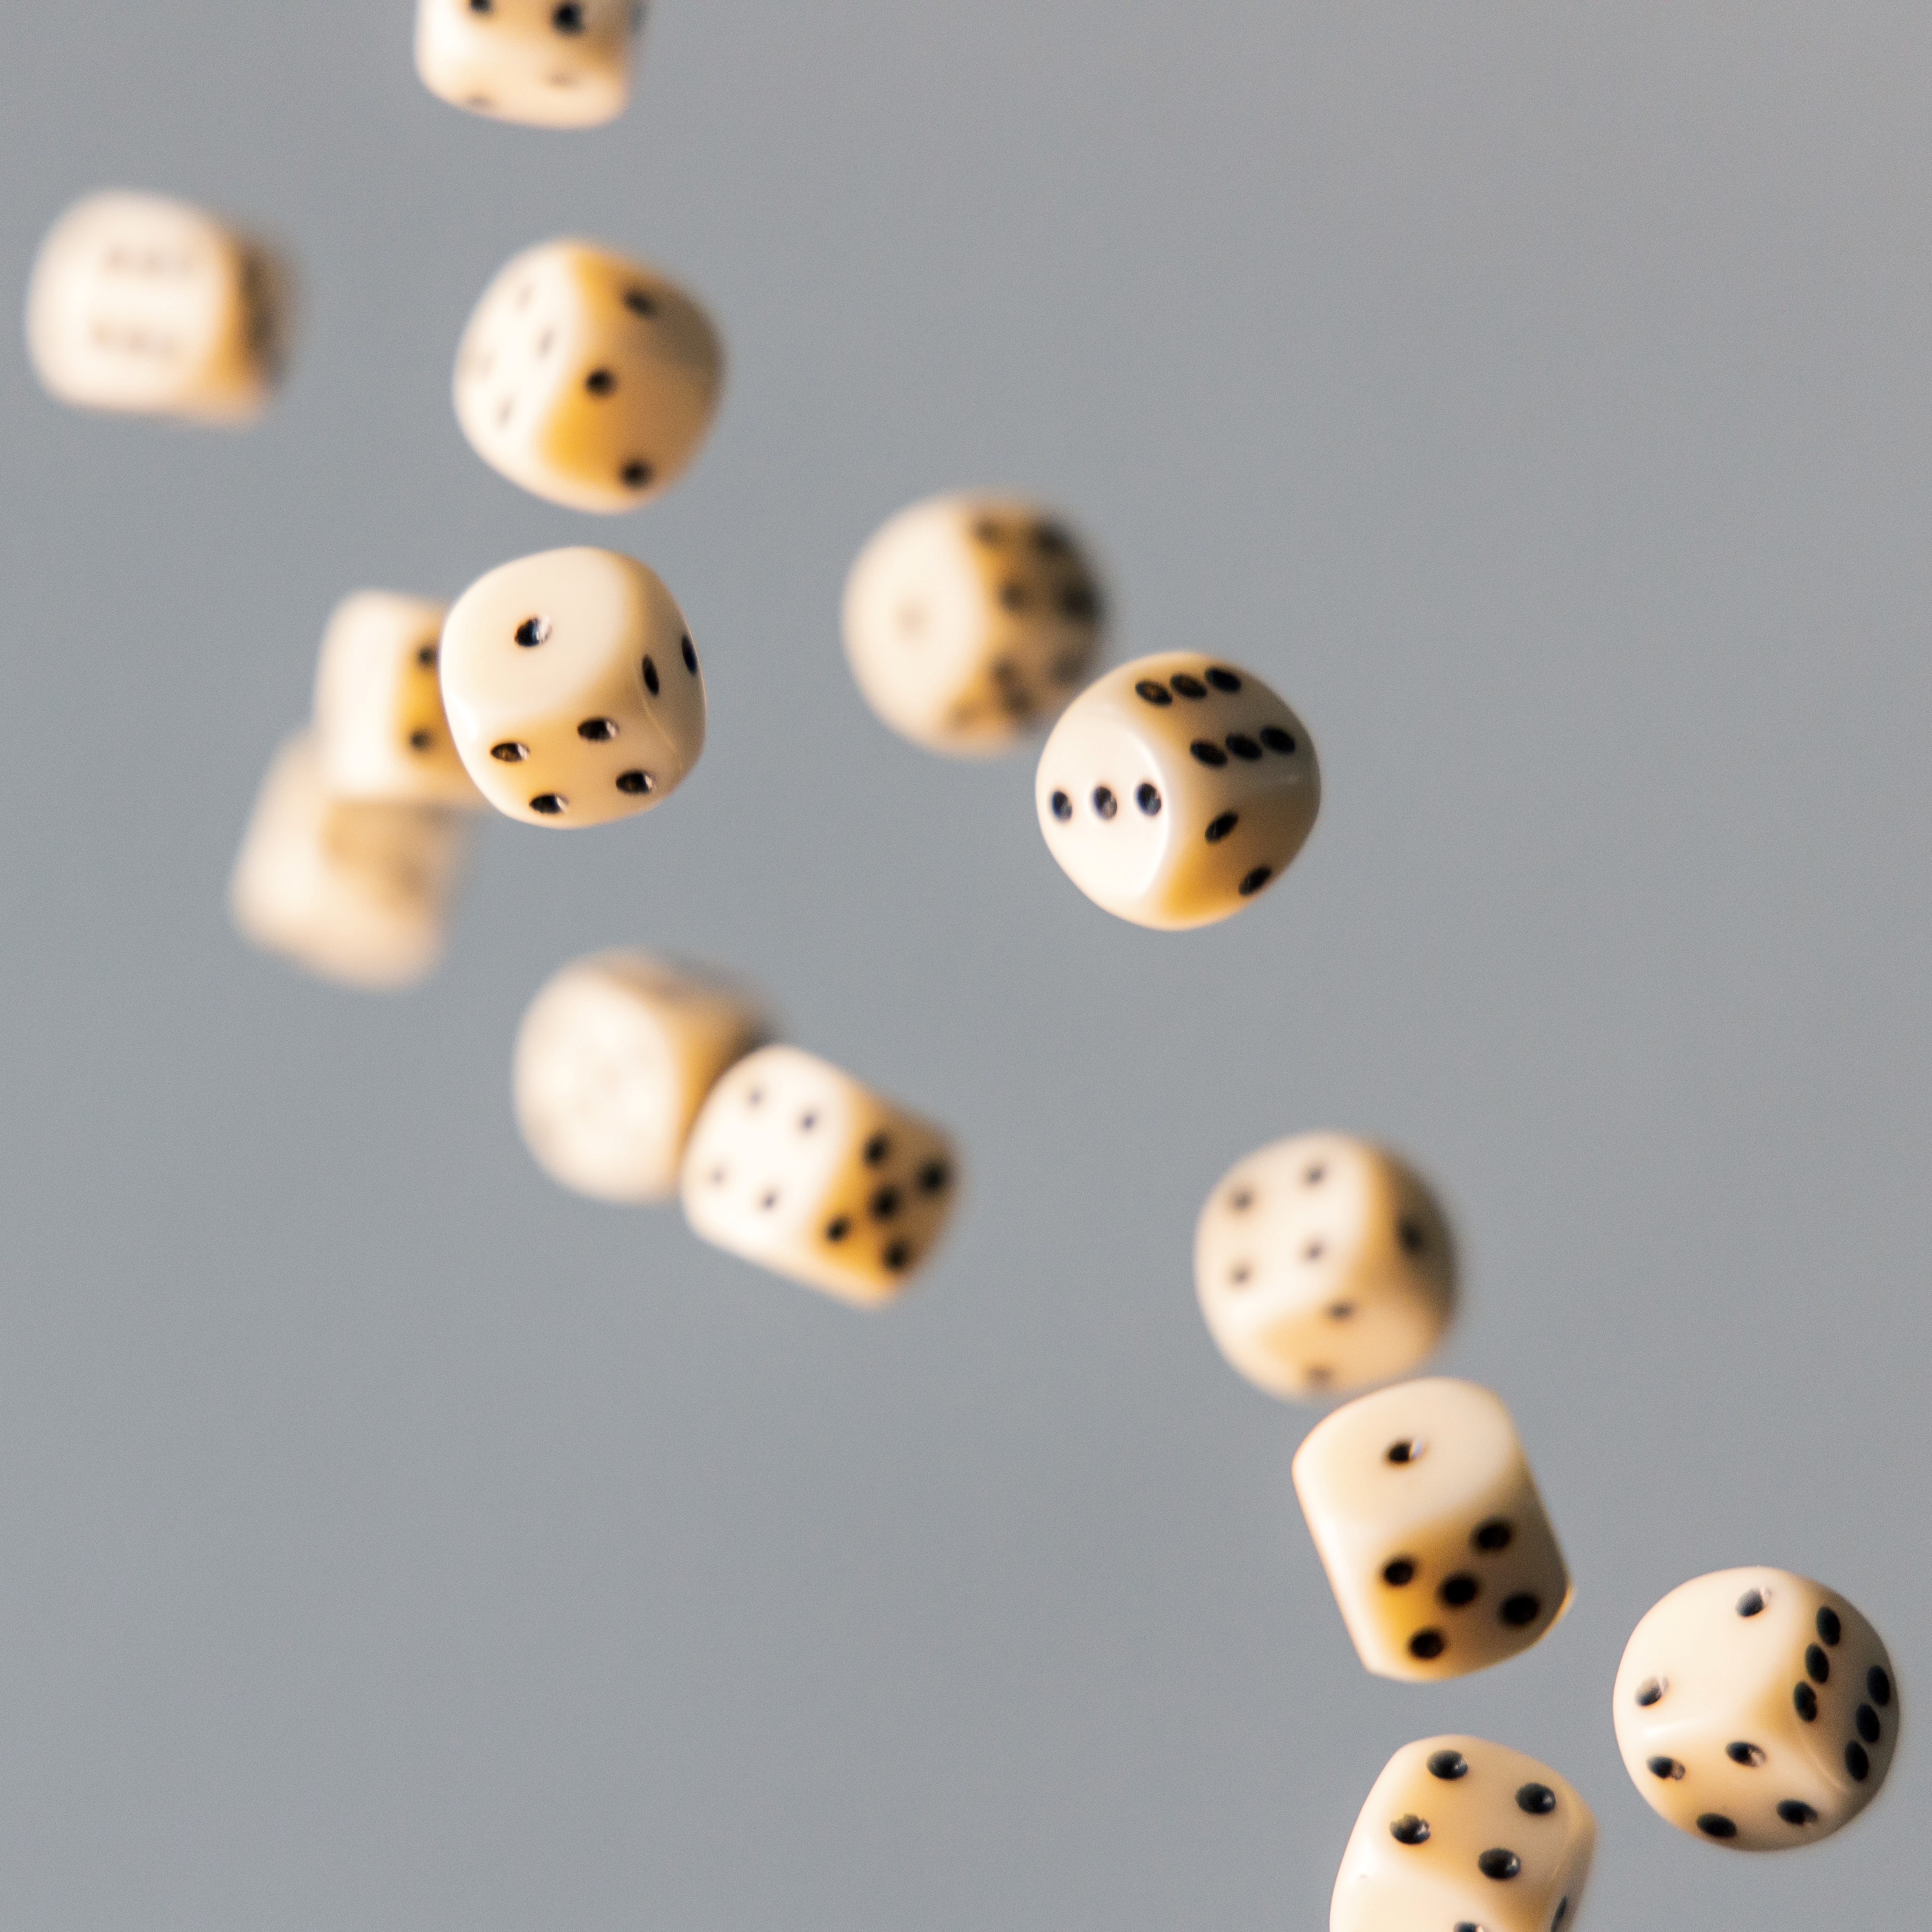
\includegraphics[width=\linewidth]{figures/dice_square.jpg}
  \colorbox{imperialorange}{\makebox[\linewidth][c]{\shortstack[c]{\vspace{0.5in}}}} \\[4ex]
  % \vfill
  % \vskip-2ex
  % \hspace{4em}
  % \parbox{0.7\textwidth}{\bfseries\Huge Core Probability Theory \par}
  % \vfill
  % \vspace{-1.0cm}
  % \setstretch{2.5}
  % \hspace{2.5em}
  \begin{center}
  \begin{minipage}[l]{0.25\linewidth}
     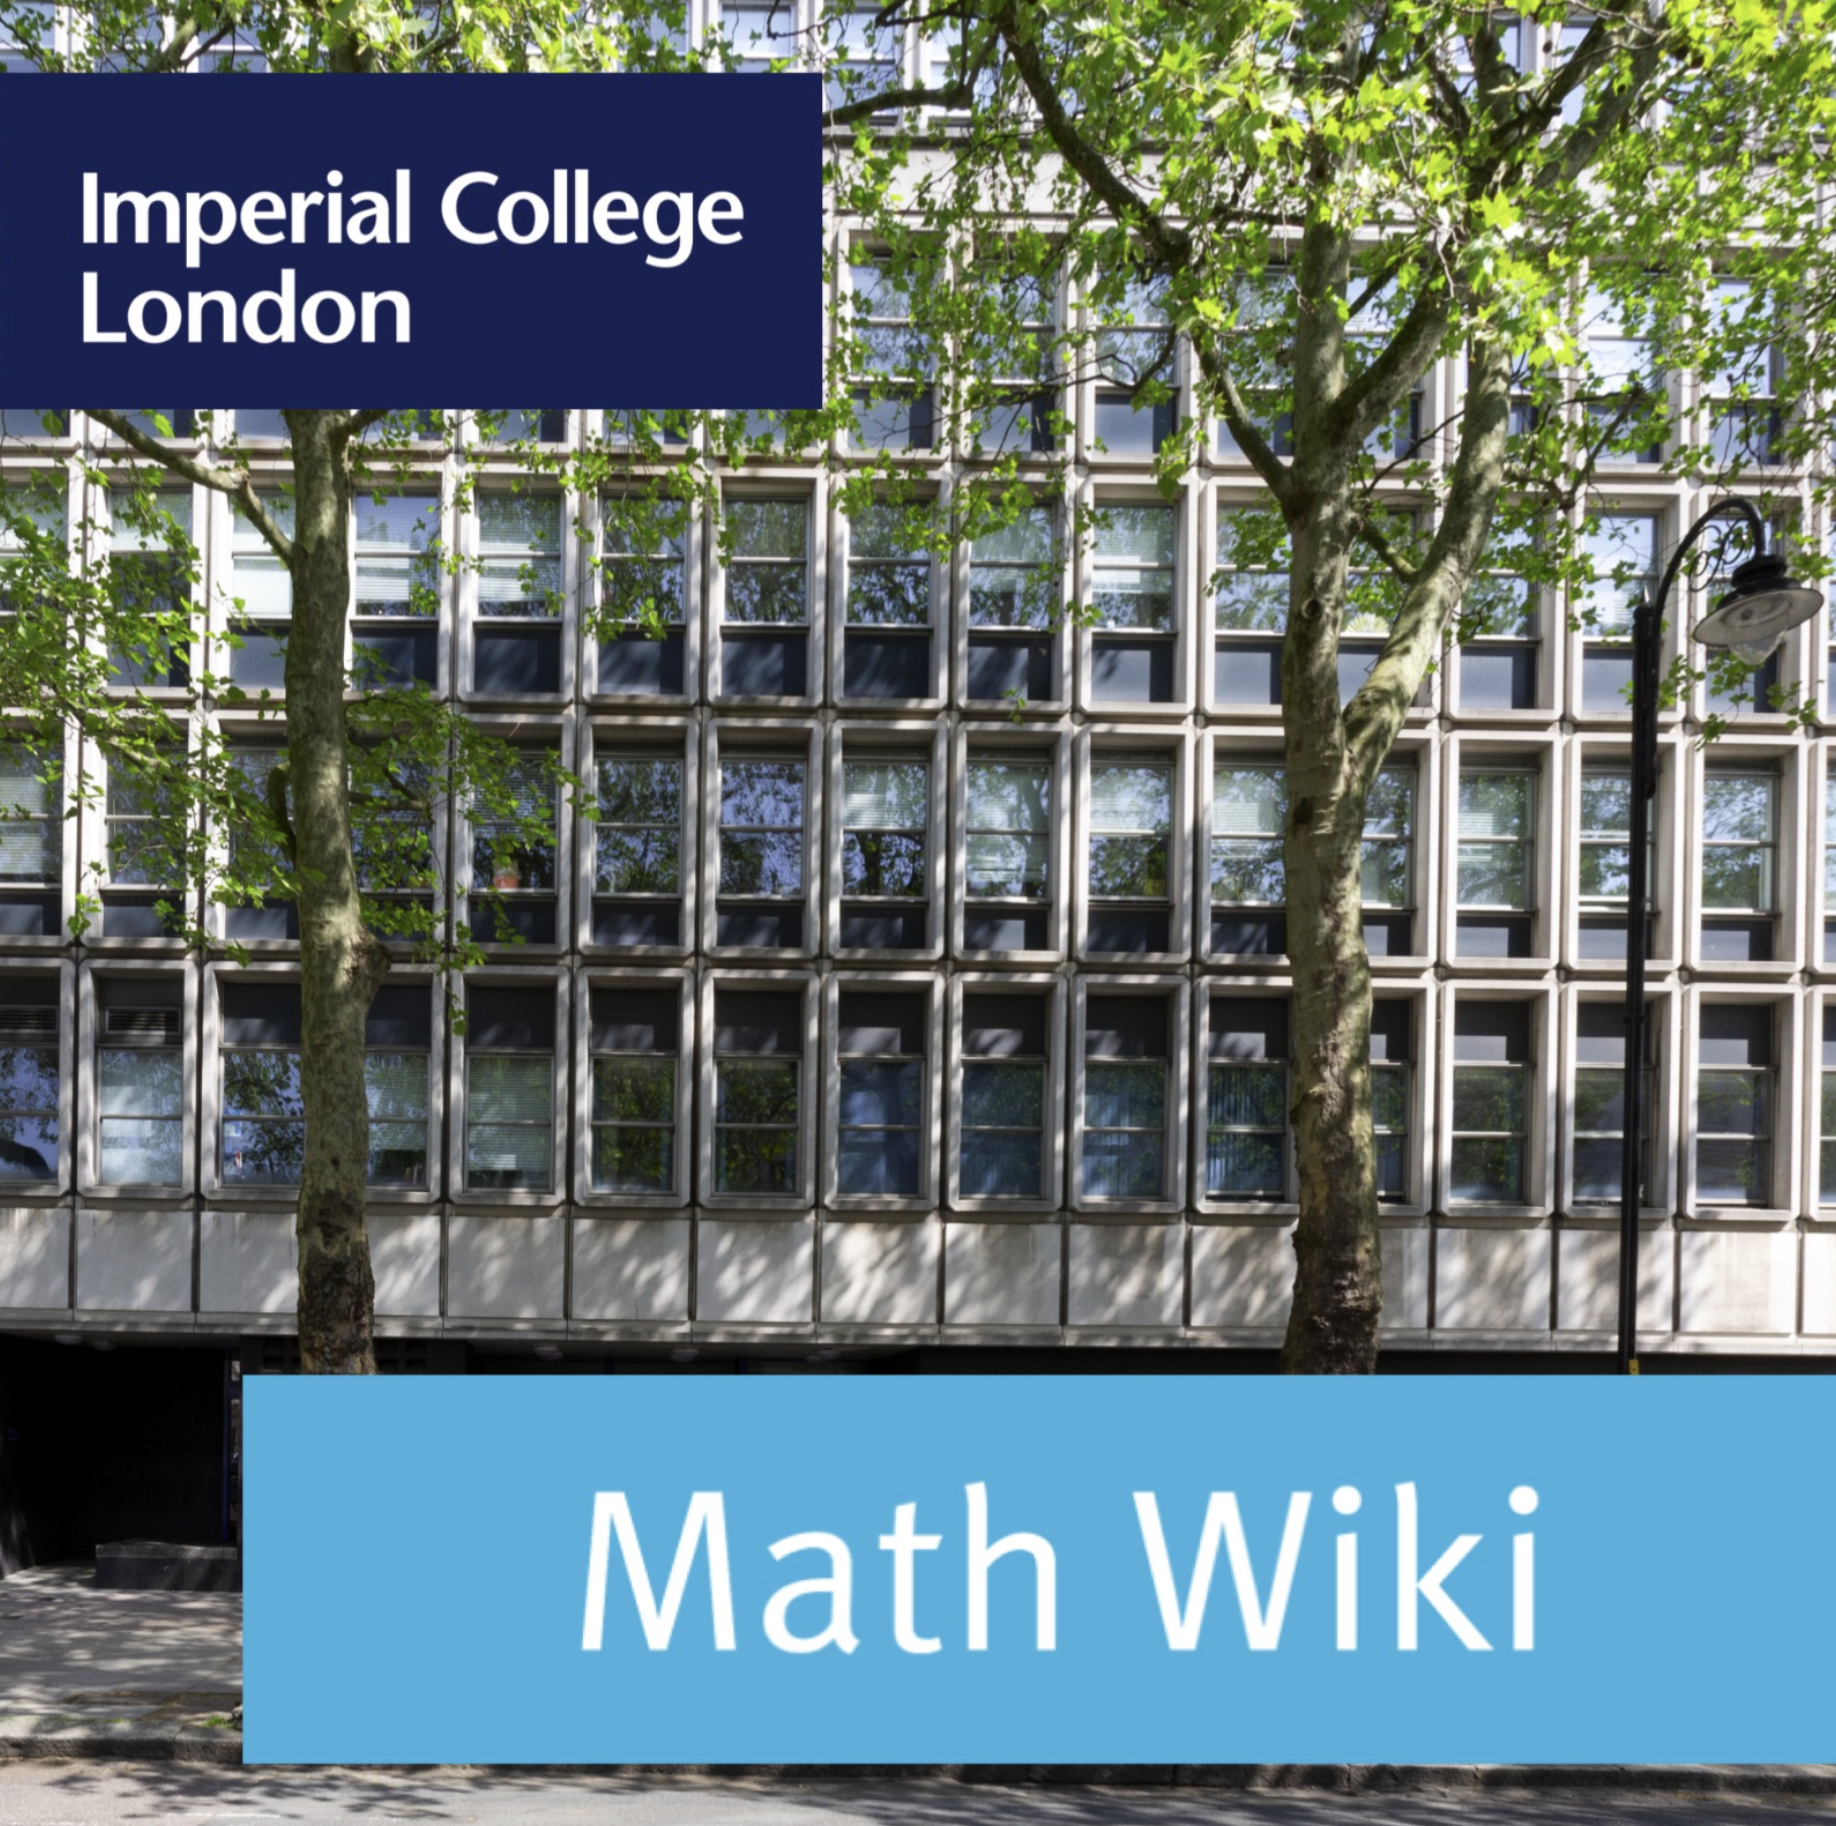
\includegraphics[width=.8\textwidth, right]{figures/mathswiki.png}
  \end{minipage}
  \hspace{.05\linewidth}
  \begin{minipage}[l]{0.5\linewidth}
    {\sffamily {\bfseries \Huge Probability Theory} \\[.5ex]
    {\Large With introductions to stochastic processes} \\[.5ex]
    {\normalsize Written as part of the Imperial College MathsWiki project.} \\[4ex]
    \textit{\large Ivan Kirev and Samuel Lam} \\[1ex]
    Version: 0.1.7 (Date: \today)}
  \end{minipage}
  \end{center}
\end{titlepage}

\restoregeometry
\newpage 

\thispagestyle{empty}
\phantom{This page has been left intentionally blank.}
\newpage